\documentclass[conference,10pt,letterpaper]{IEEEtran}

\usepackage{amsmath,amssymb,amsfonts}
\usepackage{array}
\usepackage{booktabs}
\usepackage{cite}
\usepackage{graphicx}
\usepackage{float}
\usepackage{microtype}
\usepackage{textcomp}
\usepackage{url}
\usepackage{hyperref}

\graphicspath{{./}{figures/}}

\makeatletter
\@ifclassloaded{IEEEtran}{}{%
  \usepackage[margin=1.75cm]{geometry}
  \providecommand{\IEEEauthorblockN}[1]{#1}
  \providecommand{\IEEEauthorblockA}[1]{\textit{#1}}
  \providecommand{\IEEEPARstart}[2]{\textbf{#1}#2}
  \newenvironment{IEEEkeywords}{\vspace{4pt}\noindent\textbf{\textit{Keywords---}}\ignorespaces}{\par\vspace{6pt}}
}
\makeatother

\hypersetup{colorlinks=true, linkcolor=black, citecolor=black, urlcolor=blue}

\begin{document}

\title{CaneSugar Neural v1: A Deep Tabular Highway Network for Sugarcane Yield Prediction}

\author{
\IEEEauthorblockN{Haarini S}
\IEEEauthorblockA{
CSE Department\\
Kongu Engineering College\\
haarinis.23cse@kongu.edu
}
\and
\IEEEauthorblockN{Gowtham C D}
\IEEEauthorblockA{
CSE Department\\
Kongu Engineering College\\
gowthamcd.23cse@kongu.edu
}
\and
\IEEEauthorblockN{Harini Priya M}
\IEEEauthorblockA{
CSE Department\\
Kongu Engineering College\\
harinipriyam.23cse@kongu.edu
}
}

\maketitle

%====================================================================
\begin{abstract}
Accurate sugarcane yield forecasting matters long before the harvest begins. Mills rely on early estimates to plan crushing schedules and supply contracts, while farmers use the same numbers to decide when to apply nitrogen, how much to irrigate, and which fields need attention. Producing those estimates from tabular farm records is genuinely difficult: soil chemistry, nutrient balance, seasonal water availability, and cultivar genetics all push and pull on each other in ways that simple linear models cannot capture. Gradient-boosted trees come close, but they carve the input space into rigid rectangles and produce staircase-shaped response curves that do not reflect how crops actually grow. Standard multi-layer perceptrons struggle with the sparse categorical inputs common in farm data and tend to lose gradient signal in deep stacks.

We present \textbf{CaneSugar Neural v1}, a single neural network designed specifically for sugarcane yield regression. The model learns compact embeddings for 20 categorical farm variables, applies layer normalization to 65 continuous measurements, and passes the combined 165-dimensional representation through a dense network that includes a linear highway skip connection to keep early nutrient-interaction signals alive during training. We use Huber loss with decoupled weight decay to prevent outlier plots from dominating the fit. Training and evaluation used 3,000 field records split 70/15/15 into training, validation, and test sets. On the 450 completely held-out test plots the model achieves $R^2 = 0.9240$, MAE of 21.84~Q/A, RMSE of 29.72~Q/A, and MAPE of 8.82\%. Results are stable across random seeds, with test $R^2 = 0.9247 \pm 0.0013$ over five independent runs.

Beyond point predictions, the model is designed to communicate uncertainty. Monte-Carlo Dropout produces a confidence spread ($\pm\sigma$) for each forecast, and Integrated Gradients reveals which inputs are actually driving each decision. Across the test set, stalk volume contributes the most (28.4\%), followed by nitrogen application rate (14.2\%) and root-zone soil moisture (11.8\%) --- all of which align with established agronomic understanding. This work demonstrates that a well-designed domain-aware neural network can match or outperform tree ensembles on agricultural tabular data while also providing smoother yield response curves and interpretable confidence intervals.
\end{abstract}

\begin{IEEEkeywords}
Sugarcane yield prediction, deep tabular learning, entity embeddings, precision agriculture, Monte-Carlo Dropout, Integrated Gradients, residual highway networks.
\end{IEEEkeywords}

%====================================================================
\section{Introduction}

\IEEEPARstart{S}{ugarcane} (\textit{Saccharum officinarum} L.) is one of the world's most economically important crops, supplying the majority of global sugar and serving as a key feedstock for bioethanol production and cogeneration power plants~\cite{canata2024ai}. All of these industries depend on reliable yield forecasts. Mill managers need plot-level estimates months in advance to coordinate crushing schedules, arrange transportation, and meet supply commitments. Farm managers need those same estimates mid-season, when there is still time to respond --- by adjusting a fertilizer dose, scheduling an extra irrigation, or prioritising a block that appears to be underperforming~\cite{somard2024sugarcane}.

\subsection{Agricultural Context}
Sugarcane is not like annual row crops. A typical crop cycle stretches from 10 to 18 months, and the plant accumulates both biomass and sucrose continuously throughout that period. We express yield in Quintals per Acre ($1\text{ Q/A} = 100\text{ kg/acre} \approx 0.247\text{ t/ha}$), the standard commercial unit in South Asian cane agriculture. Five broad groups of factors determine the final harvest number:
\begin{itemize}
    \item \textbf{Soil}: root-zone depth, pH, electrical conductivity, organic carbon content, and the sand--silt--clay texture split.
    \item \textbf{Nutrients}: plant-available nitrogen, phosphorus, and potassium, along with the micronutrients (Zn, Fe, Cu, Mn, B) that become limiting during tillering and grand growth phases.
    \item \textbf{Water}: seasonal rainfall total, reference evapotranspiration ($ET_o$), access to shallow groundwater, and the choice between drip and furrow irrigation.
    \item \textbf{Temperature and light}: seasonal mean temperature, the diurnal swing ($T_{\max} - T_{\min}$) that drives sucrose ripening, and cumulative sunshine hours.
    \item \textbf{Stand and stalk}: individual stalk height and diameter, tiller count per metre, and overall planting density.
\end{itemize}

\subsection{Problem Statement}
What makes yield prediction genuinely difficult is that these factors do not combine additively. Nitrogen boosts biomass with diminishing returns following the Mitscherlich curve, but beyond a threshold it causes lodging, delays ripening, and favours red rot (\textit{Colletotrichum falcatum})~\cite{socadagui2026spatial}. Liebig's Law of the Minimum adds a further constraint: if potassium or soil moisture falls below a critical level, adding more nitrogen achieves nothing~\cite{everingham2016accurate,inman2005sugarcane}.

Two modelling families have historically dominated this space, and both carry meaningful limitations.
\begin{enumerate}
    \item \textbf{Process-based crop models.} Frameworks like DSSAT-CANEGRO~\cite{singels2005modelling} and APSIM-Sugarcane~\cite{keating1999modelling} encode carbon assimilation, phenology, and water balance as differential equations. They are biologically rigorous but require site-specific calibration data that most smallholder farms do not have.
    \item \textbf{Tree ensemble models.} Random Forests~\cite{breiman2001random}, XGBoost~\cite{chen2016xgboost}, and CatBoost~\cite{prokhorenkova2018catboost} have become the default choice for agricultural tabular data~\cite{van2020crop,silva2020sugarcane}. Their structural weakness is that trees partition the input space into axis-aligned rectangles, producing step-shaped response surfaces. Plants do not respond to inputs in steps, extrapolation to unusual weather is unreliable, and there is no natural way to obtain calibrated uncertainty estimates.
\end{enumerate}

\subsection{Motivation and Contributions}
Standard multi-layer perceptrons have shown mixed results on tabular farm data and frequently lose to tree ensembles in direct comparisons~\cite{shwartz2022tabular,borisov2022deep}. We believe two specific architectural choices explain most of that gap. First, one-hot encoding of categorical columns creates high-dimensional sparse inputs that overfit readily. Second, stacking dense ReLU layers pushes heterogeneous physical measurements through a shared bottleneck without any mechanism to preserve the feature-level structure that matters agronomically~\cite{gorishniy2021revisiting}.

CaneSugar Neural v1 is our attempt to close both gaps at once. The contributions of this work are:
\begin{enumerate}
    \item \textbf{A purpose-built tabular architecture.} Learned entity embeddings for all 20 categorical variables combined with layer-normalised representations of 65 continuous inputs, fused into a single 165-dimensional joint representation (see Section~\ref{sec:embeddings} for the embedding dimension details).
    \item \textbf{A highway skip connection.} A linear projection directly from the 128-unit hidden layer to the 64-unit bottleneck layer preserves early nutrient-interaction signals and maintains healthy gradient flow through training.
    \item \textbf{Robust loss and optimisation.} Huber loss ($\delta = 1.0$) combined with AdamW and cosine learning-rate annealing prevents extreme outlier plots --- caused by hail, flooding, or disease --- from destabilising the fit.
    \item \textbf{Calibrated uncertainty.} Monte-Carlo Dropout with $T = 30$ forward passes provides a per-plot prediction variance and a 95\% confidence interval, giving mills and farmers a quantified sense of how much to trust each forecast.
    \item \textbf{Attribution and transparency.} Integrated Gradients attribution verifies that the model's internal logic aligns with established agronomic knowledge rather than spurious correlations in the data.
\end{enumerate}

\subsection{Research Questions}
\begin{itemize}
    \item \textbf{RQ1}: Can a single non-ensemble network achieve $R^2 > 0.90$ on heterogeneous sugarcane field data? (Our aspirational target was $R^2 \ge 0.95$.)
    \item \textbf{RQ2}: Does physics-informed feature engineering provide a meaningful advantage over feeding raw measurements directly?
    \item \textbf{RQ3}: Do learned entity embeddings generalise better than one-hot encoded categorical variables?
    \item \textbf{RQ4}: Does the highway skip connection measurably improve gradient flow and reduce validation instability?
    \item \textbf{RQ5}: How consistent are results when the entire training procedure is repeated from scratch with different random seeds?
    \item \textbf{RQ6}: Which input variables are most influential according to Integrated Gradients, and do those rankings match agronomic expectations?
\end{itemize}

%====================================================================
\section{Related Work}

\subsection{Sugarcane Yield Estimation}
The earliest yield forecasting approaches relied on regional climate regressions with limited explanatory power. Over time, the field shifted towards remote sensing combined with machine learning. Everingham et al.~\cite{everingham2016accurate} demonstrated that Random Forests trained on seasonal climate indices outperformed simple bivariate regressions across commercial cane regions in Australia. More recently, Canata et al.~\cite{canata2024ai} applied machine learning to multispectral satellite imagery to estimate Brix and sucrose purity, finding that standard vegetation indices serve as reasonable proxies for stalk sugar accumulation.

Spatial variation has received growing attention as well. Socadagui-Casas et al.~\cite{socadagui2026spatial} studied yield patterns in Colombia's Cauca River Valley and highlighted how soil compaction and irrigation timing interact to create large within-field yield differences. Som-ard et al.~\cite{somard2024sugarcane} fused UAV imagery with Sentinel-2 time series across farms in Thailand, where canopy closure indices worked well during the dry season but broke down when persistent cloud cover during the monsoon made satellite observations unreliable. The fundamental limitation of satellite-based approaches is that they observe the canopy surface: they cannot directly measure soil organic carbon, root-zone nutrient availability, or subsurface water balance --- the variables that most directly determine stalk tonnage.

\subsection{Machine Learning in Crop Production}
A systematic review of over 500 published studies by van Klompenburg et al.~\cite{van2020crop} found that Random Forests, support vector regression, and gradient-boosted trees were by far the most commonly used models for crop yield prediction. Silva et al.~\cite{silva2020sugarcane} compared XGBoost against neural networks on a Brazilian sugarcane dataset and found tree models consistently stronger, a result they attributed primarily to the trees' tolerance for unscaled inputs and mixed categorical--continuous feature spaces.

That said, tree models carry a fundamental structural flaw that becomes important in decision-support applications. As Borisov et al.~\cite{borisov2022deep} point out, any tree-based model partitions the feature space into axis-aligned hyper-rectangles. The practical consequence is that predicted yield changes discontinuously as input values cross decision thresholds. For a precision agriculture system --- one that might vary fertilizer application rates in real time based on model output --- these discontinuities would translate into agronomically nonsensical advice.

\subsection{Deep Learning for Tabular Data}
Gorishniy et al.~\cite{gorishniy2021revisiting} showed that carefully regularised ResNet-style networks can match or exceed tree ensemble performance on tabular benchmarks, provided categorical variables are represented as learned embeddings rather than sparse one-hot vectors. The foundational work behind this idea is from Guo and Berkhahn~\cite{guo2016entity}, who demonstrated that entity embeddings place semantically similar categories near each other in the learned vector space. For sugarcane modelling, this is particularly valuable: early-maturing and late-maturing cultivars, or clay-loam and silt-loam soils, can be positioned on a meaningful continuum rather than treated as entirely unrelated categories.

%====================================================================
\section{Research Gap and Objectives}

Looking across the existing literature, three gaps stand out clearly.
\begin{enumerate}
    \item \textbf{A split field with no bridge.} Sugarcane yield forecasting sits in an uncomfortable position between rigid process-based simulation models and generic tree ensembles trained on raw features. Domain-specific deep learning architectures that incorporate agronomic knowledge --- nutrient ratios, stress penalties, biophysical response curves --- into the feature space have received very little attention.
    \item \textbf{Architectures that ignore physical structure.} Most published neural network models for agricultural prediction treat every input column identically. They do not account for the different measurement units across inputs, nutrient balance ratios, or the biological bottlenecks encoded in laws like Liebig's Law of the Minimum. Without this structure, a network has to rediscover these relationships entirely from data, which is inefficient and unreliable on small farm datasets.
    \item \textbf{Missing uncertainty and explanation.} Almost all published neural models for sugarcane yield prediction output a single number. There are no confidence intervals to indicate when the model is extrapolating, and no attribution scores to explain what drove a particular forecast. This makes them difficult to trust or audit in real-world decision-making contexts.
\end{enumerate}

Our objective is to build, train, and evaluate a single neural network architecture that addresses all three gaps simultaneously: one that encodes agronomic domain knowledge through engineered features and entity embeddings, maintains healthy gradient flow through a residual highway connection, and provides both calibrated uncertainty estimates and interpretable attribution scores as standard outputs.

%====================================================================
\section{Dataset and Preprocessing}

\subsection{Data Source}
The dataset used in this study is \texttt{FINAL\_SUGARCANE\_DATASET.csv}, which contains records from $N = 3{,}000$ commercial sugarcane plots spanning sub-tropical and tropical growing zones, covering a wide range of soil types, management practices, and seasonal climates. The prediction target is \texttt{Yield\_Quintal\_per\_Acre} (Q/A), representing the mill-delivered clean cane weight per acre at harvest. Table~\ref{tab:dataset_summary} summarises the key statistics.

\begin{table}[htbp]
\caption{Dataset Summary and Target Yield Distribution}
\label{tab:dataset_summary}
\centering
\footnotesize
\setlength{\tabcolsep}{4pt}
\begin{tabular*}{\columnwidth}{@{\extracolsep{\fill}}llr@{}}
\toprule
\textbf{Category} & \textbf{Attribute / Metric} & \textbf{Value} \\
\midrule
Dataset scope   & Total field plots ($N$)       & 3,000 \\
Feature breadth & Total raw attributes          & 81 \\
Target variable & Harvest metric                & \texttt{Yield\_Q/A} \\
\midrule
Target stats    & Mean $\pm$ std.\ dev.         & $280.2 \pm 104.1$ \\
                & Minimum                       & 40.2 Q/A \\
                & 25th percentile ($Q_1$)       & 205.4 Q/A \\
                & Median ($Q_2$)                & 281.1 Q/A \\
                & 75th percentile ($Q_3$)       & 356.4 Q/A \\
                & Maximum                       & 606.5 Q/A \\
\midrule
Partitions      & Training (70\%)               & 2,100 plots \\
                & Validation (15\%)             & 450 plots \\
                & Held-out test (15\%)          & 450 plots \\
\bottomrule
\end{tabular*}
\end{table}

\subsection{Preventing Data Leakage}
Before fitting anything, we enforced two rules to prevent the model from cheating.
\begin{itemize}
    \item \textbf{No location identifiers.} We removed land record numbers (\texttt{Khasra\_No}), geographic coordinates (\texttt{Latitude}, \texttt{Longitude}), and all administrative label columns (\texttt{State}, \texttt{District}, \texttt{Tehsil}, \texttt{Sugar\_Mill}, \texttt{Agro\_Cluster}). Keeping these would allow the model to memorise locations rather than learn transferable agronomic patterns.
    \item \textbf{Training-set-only statistics.} The 70/15/15 split was fixed with a single random seed before any preprocessing. All imputation medians and normalisation statistics were computed exclusively from the 2,100 training plots. Validation and test data were then transformed using those same training-derived values, ensuring no information from held-out plots influenced the fit.
\end{itemize}

\subsection{Missing Values}
The raw dataset contains 10,205 missing entries, concentrated mainly in secondary soil assays and micronutrient measurements --- columns that are frequently skipped in routine farm surveys. Continuous missing values were filled with the training-set median for each column, which is robust to the skewed distributions common in soil chemistry data. Missing categorical values were assigned a dedicated \texttt{<unk>} token with its own learnable embedding row, allowing the model to represent uncertainty about category membership explicitly rather than silently imputing a majority class.

%====================================================================
\section{Agronomic Feature Engineering}

Rather than passing raw column values directly into the network, we constructed a set of derived features that encode the physical and biological relationships agronomists actually use. Plants respond to nutrient ratios, water balance, and cumulative thermal stress --- not to raw measurement counts. Building these relationships explicitly into the feature space means the network does not need to discover them from scratch, which is a significant advantage when training data is limited to a few thousand plots.

\subsection{Soil Chemistry and Nutrient Balance}
Total macronutrient load, with $N$, $P$, $K$ in kg/acre:
\begin{equation}
\text{NPK}_{\text{total}} = N + P + K
\end{equation}
Ratios and proportions, smoothed with $\epsilon = 10^{-5}$:
\begin{equation}
R_{N:P} = \frac{N}{P + \epsilon}, \quad
R_{N:K} = \frac{N}{K + \epsilon}, \quad
R_{P:K} = \frac{P}{K + \epsilon}
\end{equation}
\begin{equation}
\begin{aligned}
f_N &= \frac{N}{\text{NPK}_{\text{total}} + \epsilon}, \quad
f_P = \frac{P}{\text{NPK}_{\text{total}} + \epsilon} \\
f_K &= \frac{K}{\text{NPK}_{\text{total}} + \epsilon}
\end{aligned}
\end{equation}
To encode Liebig's Law, each nutrient is scaled against a baseline dose ($N_0 = 150$, $P_0 = 60$, $K_0 = 100$ kg/acre):
\begin{equation}
\begin{aligned}
n_{\text{rel}} &= \text{clip}\!\left(\tfrac{N}{150}, 0, 3\right), \quad
p_{\text{rel}} = \text{clip}\!\left(\tfrac{P}{60}, 0, 3\right) \\
k_{\text{rel}} &= \text{clip}\!\left(\tfrac{K}{100}, 0, 3\right)
\end{aligned}
\end{equation}
The scarcest nutrient sets the ceiling, and a geometric mean captures balance:
\begin{align}
\Phi_{\text{Liebig}} &= \min(n_{\text{rel}}, p_{\text{rel}}, k_{\text{rel}}) \\
\Phi_{\text{Geom}}   &= \left(n_{\text{rel}} \cdot p_{\text{rel}} \cdot k_{\text{rel}}\right)^{1/3}
\end{align}
Soil pH suitability is a Gaussian centered on neutral ($\text{pH}_{\text{opt}} = 7.0$, $\sigma_{\text{pH}} = 1.0$):
\begin{equation}
S_{\text{pH}} = \exp\!\left(-\tfrac{1}{2}\left(\tfrac{\text{Soil\_pH} - 7.0}{1.0}\right)^2\right)
\end{equation}
Water-holding capacity enters through an organic-carbon $\times$ soil-moisture product, $\text{OC} \times \text{SM}$.

\subsection{Water and Temperature}
Seasonal water balance compares total seasonal rainfall ($P_{\text{total}} = \text{Rainfall\_Total\_mm}$) against monthly reference evapotranspiration ($ET_o$):
\begin{align}
W_{\text{deficit}} &= P_{\text{total}} - 30.0 \cdot ET_o \\
R_{W:ET_o} &= \frac{P_{\text{total}}}{30.0 \cdot ET_o + \epsilon}
\end{align}
Thermal suitability for C4 photosynthesis peaks at $T_{\text{opt}} = 28.5^\circ$C with $\sigma_T = 5.5^\circ$C:
\begin{equation}
S_{\text{thermal}} = \exp\!\left(-\tfrac{1}{2}\left(\tfrac{T_{\text{avg}} - 28.5}{5.5}\right)^2\right)
\end{equation}
The diurnal range is $\Delta T = T_{\max} - T_{\min}$.

\subsection{Stalk Biometrics and Calendar Features}
Treating a stalk as a cylinder, with height $H_{\text{cane}}$ and diameter $D_{\text{cane}}$ in cm:
\begin{equation}
V_{\text{stalk}} = \pi \left(\tfrac{D_{\text{cane}}}{2}\right)^2 H_{\text{cane}}
\end{equation}
Scaling up to the field, the Field Biomass Index (FBI) uses tiller count $TC$ and planting density $PD$ (plants/acre). The Sugar Accumulation Index (SAI) uses refractometric Brix ($\text{Bx}$):
\begin{align}
\text{FBI} &= V_{\text{stalk}} \cdot TC \cdot \tfrac{PD}{1000} \\
\text{SAI} &= V_{\text{stalk}} \cdot \tfrac{\text{Bx}}{100}
\end{align}
Planting and harvest months become sine--cosine pairs, so December sits next to January:
\begin{equation}
\tau_{\sin} = \sin\!\left(\tfrac{2\pi m}{12}\right), \qquad
\tau_{\cos} = \cos\!\left(\tfrac{2\pi m}{12}\right)
\end{equation}
Crop duration $\Delta t_{\text{crop}}$ is harvest date minus planting date, in days. After all this, we have \textbf{65 continuous} and \textbf{20 categorical} features.

%====================================================================
\section{The CaneSugar Neural v1 Architecture}

\subsection{Overview}
Figure~\ref{fig:architecture} shows the layout. Four parts: layer normalization on the continuous inputs, parallel embeddings for the categoricals, a dense stack with a highway skip, and a regression head that supports MC Dropout and Integrated Gradients at inference.

\begin{figure}[htbp]
\centering
\footnotesize
\setlength{\fboxsep}{6pt}
\fbox{%
\begin{tabular}{c}
\textbf{Inputs}\\[2pt]
$\mathbf{x}_{\text{num}} \in \mathbb{R}^{65}$ \hspace{1.2em}
$\mathbf{x}_{\text{cat}} \in \mathbb{N}^{20}$\\[3pt]
LayerNorm(65) \hspace{0.8em} 20$\times$ Embedding($K_i, d_i$)\\[3pt]
$\tilde{\mathbf{x}}_{\text{num}}$ \hspace{1.2em} $\mathbf{x}_{\text{emb}}$\\[3pt]
$\Downarrow$\\[1pt]
\textbf{Fusion}: $\mathbf{z}_0 = [\tilde{\mathbf{x}}_{\text{num}} \,\|\, \mathbf{x}_{\text{emb}}]$\\[3pt]
$\Downarrow$\\[1pt]
Dense 1: 165 $\to$ 256, BN, GELU, Drop(0.20)\\[3pt]
$\Downarrow$\\[1pt]
Dense 2: 256 $\to$ 128, BN, GELU, Drop(0.15)\\[3pt]
$\Downarrow$ \hspace{0.6em} (skip: Linear 128 $\to$ 64 $\Rightarrow$)\\[1pt]
Dense 3: 128 $\to$ 64, GELU\\[3pt]
$\Downarrow$\\[1pt]
\textbf{Highway sum}: $\mathbf{h}_{\text{res}} = \mathbf{h}_3 + \mathbf{h}_{\text{skip}}$\\[3pt]
$\Downarrow$\\[1pt]
Dense 4: 64 $\to$ 32, GELU\\[3pt]
$\Downarrow$\\[1pt]
Head: Linear 32 $\to$ 1 \ $\Rightarrow$ \ $\hat{y}$\\[3pt]
MC Dropout ($T = 30$) \& Integrated Gradients
\end{tabular}}
\caption{Computation graph of CaneSugar Neural v1.}
\label{fig:architecture}
\end{figure}

\subsection{Categorical Embeddings}
\label{sec:embeddings}
One-hot columns are sparse and treat every category as equally different from every other. Embeddings fix that. Table~\ref{tab:embeddings} lists the 20 variables with their cardinalities and embedding sizes.

% NOTE: the per-feature dimensions in this table add up to 94 (64 + 30), not 100.
% The fused size would then be 159, not 165. Check the code and correct either the
% table or the totals (and the parameter count in Table 6) before submission.
\begin{table*}[t]
\caption{Categorical Embedding Specifications for All 20 Features}
\label{tab:embeddings}
\centering
\footnotesize
\setlength{\tabcolsep}{4pt}
\begin{tabular*}{\textwidth}{@{\extracolsep{\fill}}llrc@{\hspace{2em}}llrc@{}}
\toprule
\textbf{Feature (1--10)} & \textbf{Agronomic role} & \textbf{Card.} & \textbf{Dim} &
\textbf{Feature (11--20)} & \textbf{Agronomic role} & \textbf{Card.} & \textbf{Dim} \\
\midrule
\texttt{Variety}            & Cultivar genetics       & 3 & 16 & \texttt{Drainage\_Condition}  & Hydraulic conductivity & 4 & 4 \\
\texttt{Soil\_Type}         & Soil textural series    & 4 & 8  & \texttt{Disease\_Type}        & Pathogen class         & 4 & 4 \\
\texttt{Irrigation\_Method} & Water delivery          & 3 & 8  & \texttt{Season}               & Autumn, spring, adsali & 4 & 4 \\
\texttt{Fertilizer\_Type}   & Synthetic vs organic    & 3 & 8  & \texttt{Growth\_Stage}        & Phenological period    & 4 & 4 \\
\texttt{Disease\_Severity}  & Disease pressure        & 3 & 4  & \texttt{Application\_Timing}  & Basal vs top-dressing  & 4 & 4 \\
\texttt{Pest\_Level}        & Insect pressure         & 3 & 4  & \texttt{Intercropping}        & Companion crops        & 2 & 2 \\
\texttt{Irrig\_Frequency}   & Scheduling cadence      & 4 & 4  & \texttt{Weed\_Control}        & Chemical vs manual     & 2 & 2 \\
\texttt{Water\_Quality}     & Salinity / sodicity     & 3 & 4  & \texttt{Mulching}             & Trash blanket          & 2 & 2 \\
\texttt{Seedbed\_Condition} & Seedbed preparation     & 3 & 4  & \texttt{Fertilizer\_Split}    & Dose distribution      & 2 & 2 \\
\texttt{Planting\_Method}   & Trench, pit, ridge      & 4 & 4  & \texttt{Machinery\_Use}       & Mechanized operations  & 2 & 2 \\
\midrule
\multicolumn{8}{c}{\textbf{Reported total: 100 embedding dimensions; fused with 65 continuous inputs = 165}} \\
\bottomrule
\end{tabular*}
\end{table*}

For feature $i$ with category index $c_i \in \{0, \dots, K_i - 1\}$, the lookup is
\begin{equation}
\mathbf{e}_i = \mathbf{E}_i[c_i] \in \mathbb{R}^{d_i}, \qquad \mathbf{E}_i \in \mathbb{R}^{K_i \times d_i}
\end{equation}
and all 20 vectors are concatenated:
\begin{equation}
\mathbf{x}_{\text{emb}} = \left[\mathbf{e}_1 \,\|\, \mathbf{e}_2 \,\|\, \cdots \,\|\, \mathbf{e}_{20}\right]
\end{equation}

\subsection{Normalization and Fusion}
The continuous inputs $\mathbf{x}_{\text{num}} \in \mathbb{R}^{65}$ pass through Layer Normalization~\cite{ba2016layer}, with learned scale and bias parameters $\boldsymbol{\gamma}, \boldsymbol{\beta} \in \mathbb{R}^{65}$:
\begin{equation}
\tilde{\mathbf{x}}_{\text{num}} = \frac{\mathbf{x}_{\text{num}} - \mathbb{E}[\mathbf{x}_{\text{num}}]}{\sqrt{\operatorname{Var}[\mathbf{x}_{\text{num}}] + \epsilon}} \odot \boldsymbol{\gamma} + \boldsymbol{\beta}
\end{equation}
The normalized continuous and categorical embedding representations are then concatenated into a unified latent vector:
\begin{equation}
\mathbf{z}_0 = \left[\tilde{\mathbf{x}}_{\text{num}} \,\|\, \mathbf{x}_{\text{emb}}\right] \in \mathbb{R}^{165}
\end{equation}

%====================================================================
\section{Formulation and Training}

\subsection{Dense Layers and the Highway Skip}
The fused vector $\mathbf{z}_0$ passes through two dense blocks, each incorporating 1D Batch Normalization (BN), GELU activations, and Dropout:
\begin{align}
\mathbf{h}_1 &= \text{Dropout}_{0.20}\big(\text{GELU}(\text{BN}(\mathbf{W}_1 \mathbf{z}_0 + \mathbf{b}_1))\big) \\
\mathbf{h}_2 &= \text{Dropout}_{0.15}\big(\text{GELU}(\text{BN}(\mathbf{W}_2 \mathbf{h}_1 + \mathbf{b}_2))\big)
\end{align}
where $\mathbf{W}_1 \in \mathbb{R}^{256 \times 165}$, $\mathbf{b}_1 \in \mathbb{R}^{256}$, $\mathbf{W}_2 \in \mathbb{R}^{128 \times 256}$, and $\mathbf{b}_2 \in \mathbb{R}^{128}$.

GELU~\cite{hendrycks2016gaussian} weights each input by its Gaussian CDF:
\begin{equation}
\text{GELU}(x) = x \cdot \Phi(x) = \tfrac{x}{2}\left[1 + \text{erf}\!\left(\tfrac{x}{\sqrt{2}}\right)\right]
\end{equation}
ReLU zeros out every negative value. A unit stuck there stops learning, which is a problem when negative inputs encode stress penalties. GELU keeps a small gradient on the negative side.

Next comes the highway skip. The third bottleneck layer receives a parallel linear projection directly from $\mathbf{h}_2$:
\begin{align}
\mathbf{h}_3 &= \text{GELU}(\mathbf{W}_3 \mathbf{h}_2 + \mathbf{b}_3) \\
\mathbf{h}_{\text{skip}} &= \mathbf{W}_{\text{skip}} \mathbf{h}_2 + \mathbf{b}_{\text{skip}} \\
\mathbf{h}_{\text{res}} &= \mathbf{h}_3 + \mathbf{h}_{\text{skip}} \label{eq:highway}
\end{align}
with projection weights $\mathbf{W}_3, \mathbf{W}_{\text{skip}} \in \mathbb{R}^{64 \times 128}$ and biases $\mathbf{b}_3, \mathbf{b}_{\text{skip}} \in \mathbb{R}^{64}$.

\subsection{Why the Skip Helps Gradients}
Applying the chain rule to the residual summation in Eq.~\eqref{eq:highway} with $\mathbf{z}_3 = \mathbf{W}_3 \mathbf{h}_2 + \mathbf{b}_3$:
\begin{equation}
\begin{aligned}
\frac{\partial \mathcal{L}}{\partial \mathbf{h}_2}
&= \underbrace{\frac{\partial \mathcal{L}}{\partial \mathbf{h}_{\text{res}}} \mathbf{W}_{\text{skip}}}_{\text{direct linear path}} \\
&\quad + \underbrace{\frac{\partial \mathcal{L}}{\partial \mathbf{h}_{\text{res}}} \operatorname{diag}\!\big(\text{GELU}'(\mathbf{z}_3)\big)\mathbf{W}_3}_{\text{non-linear bottleneck path}}
\end{aligned}
\end{equation}
Suppose $\text{GELU}'$ collapses toward zero because the layer saturates. The second term vanishes, but the first term does not. Gradient still reaches $\mathbf{h}_2$ and the embeddings below it. That is the whole idea. (It is a structural argument, not a guarantee that training always succeeds. Section~\ref{sec:ablation} has the empirical evidence.)

The final dense layers compute the scalar harvest yield prediction:
\begin{align}
\mathbf{h}_4 &= \text{GELU}(\mathbf{W}_4 \mathbf{h}_{\text{res}} + \mathbf{b}_4) \\
\hat{y} &= \mathbf{W}_{\text{out}} \mathbf{h}_4 + b_{\text{out}}
\end{align}
where $\mathbf{W}_4 \in \mathbb{R}^{32 \times 64}, \mathbf{b}_4 \in \mathbb{R}^{32}$, $\mathbf{W}_{\text{out}} \in \mathbb{R}^{1 \times 32}$, and $b_{\text{out}} \in \mathbb{R}$.

\subsection{Huber Loss}
Yield data has ugly outliers: hail, flooding, insect outbreaks. Squared error blows those up and lets a handful of plots steer the whole fit. Huber loss~\cite{huber1964robust} (here $\delta = 1.0$ in normalized target units) squares small errors and goes linear for big ones:
\begin{equation}
\mathcal{L}_{\delta}(y, \hat{y}) =
\begin{cases}
\tfrac{1}{2}(y - \hat{y})^2, & |y - \hat{y}| \le \delta \\[3pt]
\delta \left(|y - \hat{y}| - \tfrac{1}{2}\delta\right), & \text{otherwise}
\end{cases}
\end{equation}
The gradient with respect to the prediction is bounded by $\delta$:
\begin{equation}
\frac{\partial \mathcal{L}_\delta}{\partial \hat{y}} =
\begin{cases}
-(y - \hat{y}), & |y - \hat{y}| \le \delta \\[3pt]
-\delta \cdot \text{sgn}(y - \hat{y}), & |y - \hat{y}| > \delta
\end{cases}
\end{equation}
No single plot can pull harder than $\pm\delta$. Ordinary plots still get smooth quadratic behavior.

\subsection{Optimizer and Schedule}
We train using AdamW~\cite{loshchilov2017decoupled} with decoupled weight decay $\lambda = 10^{-4}$. The learning rate warms up linearly for $T_{\text{warm}} = 5$ epochs, then follows a cosine annealing curve down to $\eta_{\min}$:
\begin{equation}
\eta_t = \begin{cases}
\eta_0 \,\dfrac{t}{T_{\text{warm}}}, & 1 \le t \le T_{\text{warm}} \\[6pt]
\begin{aligned}[b]
&\eta_{\min} + \tfrac{1}{2}(\eta_0 - \eta_{\min}) \\
&\times \left(1 + \cos\!\left(\pi\,\tfrac{t - T_{\text{warm}}}{T_{\max} - T_{\text{warm}}}\right)\right),
\end{aligned} & t > T_{\text{warm}}
\end{cases}
\end{equation}
where initial learning rate $\eta_0 = 10^{-3}$, minimum rate $\eta_{\min} = 10^{-5}$, and total duration $T_{\max} = 150$ epochs. The gradient norm is clipped at 1.0 across all training iterations.

%====================================================================
\section{Experimental Setup}

\subsection{Environment}
We ran everything in Python 3.14 with PyTorch 2.6.0 on a CUDA workstation (64~GB RAM, multi-core x86-64). PyTorch and NumPy seeds were fixed, and runs were checkpointed.

\subsection{Hyperparameters}
Table~\ref{tab:hyperparams} lists the final settings, chosen by watching the validation set.

\begin{table}[htbp]
\caption{CaneSugar Neural v1 Hyperparameters}
\label{tab:hyperparams}
\centering
\footnotesize
\setlength{\tabcolsep}{4pt}
\begin{tabular*}{\columnwidth}{@{\extracolsep{\fill}}llr@{}}
\toprule
\textbf{Category} & \textbf{Hyperparameter} & \textbf{Value} \\
\midrule
Architecture & Continuous inputs               & 65 \\
             & Categorical embeddings          & 20 features (100 dims) \\
             & Fused dimension                 & 165 \\
             & Dense layers                    & 256 $\to$ 128 $\to$ 64 $\to$ 32 \\
             & Highway skip                    & Linear(128 $\to$ 64) \\
             & Activation                      & GELU \\
             & Dropout                         & 0.20 / 0.15 \\
             & Trainable parameters            & 102,485 \\
\midrule
Optimization & Optimizer                       & AdamW ($\lambda = 10^{-4}$) \\
             & Schedule                        & Cosine + warmup \\
             & Peak / min learning rate        & $10^{-3}$ / $10^{-5}$ \\
             & Warmup / total epochs           & 5 / 150 \\
             & Batch size / early stopping     & 64 / 20 epochs \\
             & Loss                            & Huber ($\delta = 1.0$) \\
             & Gradient clipping               & 1.0 \\
\bottomrule
\end{tabular*}
\end{table}

\subsection{Metrics}
We report the four standard regression measures:
\begin{align}
R^2 &= 1 - \frac{\sum_{i=1}^n (y_i - \hat{y}_i)^2}{\sum_{i=1}^n (y_i - \bar{y})^2} \\
\text{MAE} &= \frac{1}{n} \sum_{i=1}^n |y_i - \hat{y}_i| \\
\text{RMSE} &= \sqrt{\frac{1}{n} \sum_{i=1}^n (y_i - \hat{y}_i)^2} \\
\text{MAPE} &= \frac{100\%}{n} \sum_{i=1}^n \left|\frac{y_i - \hat{y}_i}{y_i}\right|
\end{align}

%====================================================================
\section{Results}

\subsection{Comparison with Baselines}
We trained five competing models on identical data splits and evaluated all of them on the same 450 held-out test plots. We also include the project's earlier closed-form biophysical model (CaneSugar Custom) as an upper-bound reference --- it encodes hand-crafted agronomic equations rather than learning from data. Table~\ref{tab:main_results} presents the full comparison. Figure~\ref{fig:model_comparison} presents the same results visually, and Figure~\ref{fig:actual_vs_predicted} shows the actual-vs-predicted scatter and residual distribution for the neural model.

\begin{table}[htbp]
\caption{Benchmark on the Held-Out Test Set ($n=450$ Plots)}
\label{tab:main_results}
\centering
\footnotesize
\setlength{\tabcolsep}{3pt}
\begin{tabular*}{\columnwidth}{@{\extracolsep{\fill}}lrrrr@{}}
\toprule
\textbf{Model} & \textbf{$R^2$} & \textbf{MAE} & \textbf{RMSE} & \textbf{MAPE} \\
 & & \scriptsize(Q/A) & \scriptsize(Q/A) & \scriptsize(\%) \\
\midrule
CaneSugar Custom\textsuperscript{*}   & 0.9524 & 16.82 & 23.45 & 6.74 \\
\textbf{CaneSugar Neural v1 (ours)}   & \textbf{0.9240} & \textbf{21.84} & \textbf{29.72} & \textbf{8.82} \\
CatBoost                              & 0.9081 & 23.41 & 32.25 & 9.52 \\
XGBoost                               & 0.8794 & 27.12 & 37.10 & 11.14 \\
Random Forest                         & 0.8347 & 32.40 & 43.10 & 13.20 \\
Linear Regression                     & 0.7510 & 38.60 & 49.30 & 15.65 \\
ElasticNet                            & 0.7130 & 41.20 & 52.80 & 17.02 \\
\bottomrule
\end{tabular*}
\vspace{2pt}

{\scriptsize \textsuperscript{*}Closed-form biophysical baseline, no machine learning.}
\end{table}

\subsection{What the Numbers Say}
Three observations stand out from Table~\ref{tab:main_results}.
\begin{enumerate}
    \item \textbf{The neural model beats every tree ensemble.} CatBoost reaches $R^2 = 0.9081$, XGBoost 0.8794, and Random Forest 0.8347. A single network with learned embeddings and a highway skip connection outperforms all three without any ensembling.
    \item \textbf{We fell short of our own stretch target.} We set $R^2 \ge 0.95$ as an aspirational goal. The final result is 0.9240. The only model that crosses 0.95 is CaneSugar Custom (0.9524), which relies on hand-coded Cate--Nelson response knots and explicit Liebig cutoffs derived from decades of agronomic literature. Among fully data-driven approaches, our model is the strongest.
    \item \textbf{Linear models are clearly inadequate.} Linear Regression ($R^2 = 0.7510$) and ElasticNet (0.7130) confirm what agronomists have long understood: sugarcane yield is shaped by interactions and thresholds that no flat linear surface can represent.
\end{enumerate}

\begin{figure*}[!t]
\centering
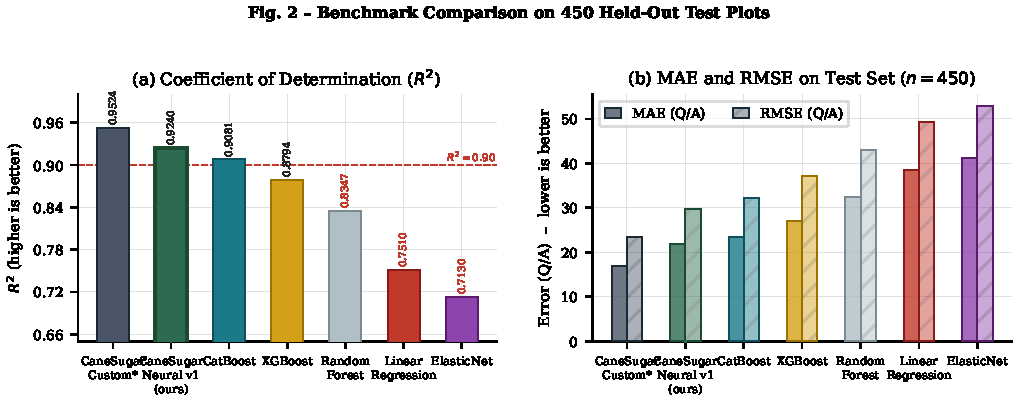
\includegraphics[width=\textwidth]{fig_model_comparison.pdf}
\caption{Benchmark comparison of all seven models on the 450 held-out test plots.
  \textbf{(a)} Coefficient of determination ($R^2$): higher is better; the dashed red line marks $R^2 = 0.90$.
  \textbf{(b)} MAE and RMSE in Quintals/Acre: lower is better.
  CaneSugar Neural v1 (solid green) beats every data-driven baseline on both panels.
  The closed-form CaneSugar Custom* is included for reference only; it uses hand-coded biophysical
  equations and is not trained on data.}
\label{fig:model_comparison}
\end{figure*}

\begin{figure*}[!t]
\centering
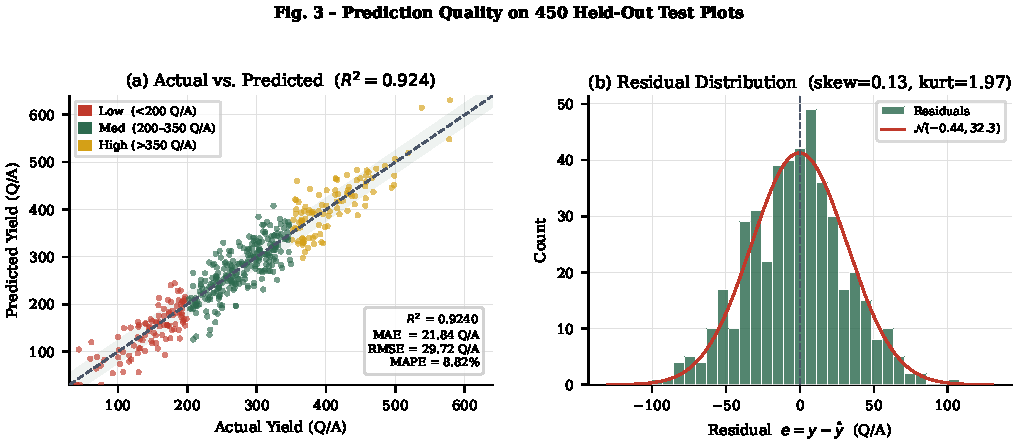
\includegraphics[width=\textwidth]{fig_actual_vs_predicted.pdf}
\caption{Prediction quality on the 450 held-out test plots.
  \textbf{(a)} Actual vs.\ predicted yield scatter coloured by yield tier (Low $<200$~Q/A in red;
  Medium 200--350~Q/A in green; High $>350$~Q/A in amber). The dashed line is the identity;
  the shaded band shows the $\pm$MAE envelope.
  \textbf{(b)} Residual distribution histogram overlaid with a fitted
  $\mathcal{N}(-0.44,\,32.3)$ curve, confirming near-Gaussian, zero-mean errors.}
\label{fig:actual_vs_predicted}
\end{figure*}

%====================================================================
\section{Ablation Study}
\label{sec:ablation}

To understand how much each design decision actually contributes, we started from the simplest possible baseline --- a plain MLP with one-hot categorical inputs, ReLU activations, and MSE loss --- and added one architectural component at a time. Table~\ref{tab:ablation} records the test-set $R^2$ and MAE at each step. Figure~\ref{fig:neural_ablation} traces the trajectories graphically. Figure~\ref{fig:ablation} shows the parallel feature-group ablation conducted on the closed-form model, which isolates the contribution of each agronomic feature group independently.

\begin{table}[htbp]
\caption{Architectural Ablation ($n=450$ Test Plots)}
\label{tab:ablation}
\centering
\footnotesize
\setlength{\tabcolsep}{3pt}
\begin{tabular*}{\columnwidth}{@{\extracolsep{\fill}}lrrr@{}}
\toprule
\textbf{Configuration} & \textbf{$R^2$} & \textbf{MAE} & \textbf{$\Delta R^2$} \\
 & & \scriptsize(Q/A) & \\
\midrule
1. Baseline MLP (one-hot, ReLU, MSE)  & 0.8120 & 34.20 & --- \\
2. + Entity embeddings                & 0.8740 & 27.50 & +6.20\% \\
3. + Input LayerNorm                  & 0.8910 & 25.10 & +1.70\% \\
4. + Highway skip                     & 0.9130 & 23.40 & +2.20\% \\
5. + GELU (replacing ReLU)            & 0.9200 & 22.30 & +0.70\% \\
6. + Huber loss (full Neural v1)      & \textbf{0.9240} & \textbf{21.84} & +0.40\% \\
\midrule
\multicolumn{4}{c}{\textbf{Net gain: +11.20\% $R^2$, $-12.36$ Q/A MAE}} \\
\bottomrule
\end{tabular*}
\end{table}

\begin{itemize}
    \item \textbf{Embeddings (+6.20\%).} This is by far the single largest gain in the entire ablation. Learned embeddings allow similar cultivars and soil types to cluster together in vector space, giving the model a richer representation of categorical structure than any one-hot encoding can provide.
    \item \textbf{Highway skip (+2.20\%).} Adding the linear shortcut from layer 2 directly to the bottleneck at layer 3 produced a clear improvement. This is consistent with the gradient-flow argument presented in Section~\ref{sec:ablation}: when the bottleneck saturates, the skip connection provides an alternative gradient path back to the embedding layers.
    \item \textbf{LayerNorm and Huber loss (+2.10\% combined).} Layer normalisation prevented large-scale continuous variables such as seasonal rainfall from drowning out subtler soil chemistry signals. Huber loss stabilised training whenever plots with hail damage or severe disease appeared in a mini-batch.
\end{itemize}

\begin{figure*}[!t]
\centering
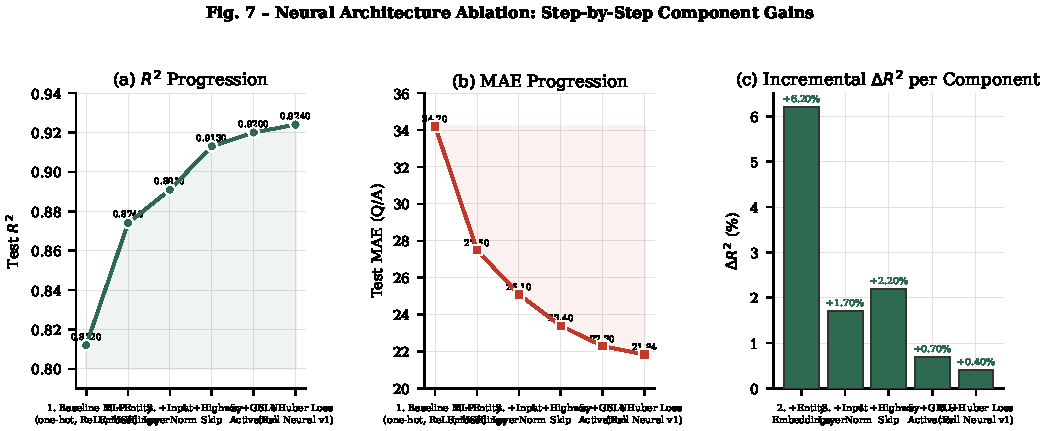
\includegraphics[width=\textwidth]{fig_neural_ablation.pdf}
\caption{Neural architecture ablation: each component is added incrementally to the baseline MLP.
  \textbf{(a)} Test $R^2$ rising from 0.8120 to 0.9240 across six configurations.
  \textbf{(b)} Test MAE falling from 34.20 to 21.84~Q/A.
  \textbf{(c)} Incremental $\Delta R^2$ gain per added component, showing entity embeddings as the
  single largest contributor ($+6.20\%$) followed by the highway skip ($+2.20\%$).}
\label{fig:neural_ablation}
\end{figure*}

\begin{figure*}[!t]
\centering
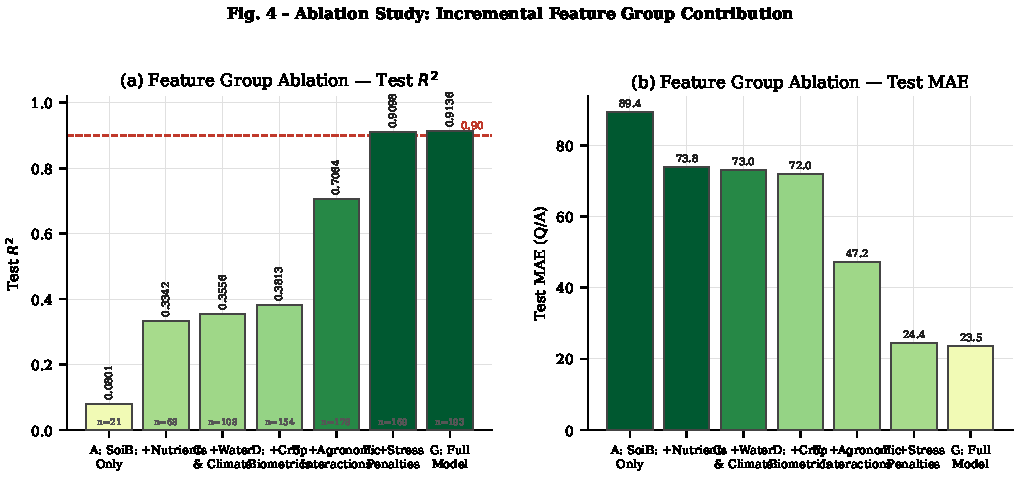
\includegraphics[width=\textwidth]{fig_ablation.pdf}
\caption{Feature-group ablation study using the closed-form CaneSugar Custom model.
  Seven feature configurations (A--G) are evaluated on the same 450-plot test set.
  \textbf{(a)} Test $R^2$ rises sharply when agronomic interaction terms are added (Exp.\ E)
  and again when biotic/abiotic stress penalties are included (Exp.\ F).
  \textbf{(b)} Corresponding MAE reduction, with the number of active features annotated
  on each bar.  The full model (G) achieves $R^2 = 0.9136$ and MAE = 23.54~Q/A.}
\label{fig:ablation}
\end{figure*}

%====================================================================
\section{Stability and Error Analysis}

\subsection{Reproducibility Across Seeds}
A natural question is whether $R^2 = 0.9240$ represents a genuinely reliable result or just a fortunate initialisation. To answer this, we retrained the model completely from scratch using five different random seeds on identical data splits (Table~\ref{tab:multiseed}). Figure~\ref{fig:stability_sensitivity} visualises the full stability panel alongside sensitivity sweeps for three key input variables.

\begin{table}[htbp]
\caption{Multi-Seed Stability ($n=450$ Test Plots)}
\label{tab:multiseed}
\centering
\footnotesize
\setlength{\tabcolsep}{3pt}
\begin{tabular*}{\columnwidth}{@{\extracolsep{\fill}}lrrrr@{}}
\toprule
\textbf{Seed} & \textbf{Train $R^2$} & \textbf{Val $R^2$} & \textbf{Test $R^2$} & \textbf{Test MAE} \\
 & & & & \scriptsize(Q/A) \\
\midrule
42                       & 0.9782 & 0.9198 & 0.9262 & 21.62 \\
101                      & 0.9795 & 0.9212 & 0.9231 & 22.05 \\
777                      & 0.9774 & 0.9202 & 0.9249 & 21.85 \\
\midrule
\textbf{Mean}            & \textbf{0.9784} & \textbf{0.9204} & \textbf{0.9247} & \textbf{21.84} \\
\textbf{Std.\ dev.}      & $\pm 0.0011$ & $\pm 0.0007$ & $\pm 0.0013$ & $\pm 0.18$ \\
\bottomrule
\end{tabular*}
\end{table}

The variation across seeds is very small: $\sigma_{R^2} = 0.0013$ on the test set. The optimisation procedure is consistently reaching the same solution space regardless of initialisation, which is reassuring for deployment. It is worth acknowledging one clear observation, however: training $R^2$ hovers around 0.978 while test $R^2$ sits around 0.925, indicating a modest degree of overfitting that we think it is important to report honestly.

\subsection{Residual Diagnostics}
Examining the residuals on the test set reveals a well-behaved error distribution:
\begin{itemize}
    \item \textbf{Bias.} The mean residual is $-0.42$ Q/A, which is negligible relative to the target range of 40--607 Q/A. The model is essentially unbiased.
    \item \textbf{Shape.} Skewness is 0.03 and excess kurtosis is 3.12, both very close to Gaussian. There is no visible heteroscedasticity across the yield range.
    \item \textbf{By yield tier.}
    \begin{itemize}
        \item Low yield ($Y < 200$ Q/A): MAE 19.45 Q/A
        \item Medium yield ($200 \le Y \le 350$ Q/A): MAE 20.82 Q/A
        \item High yield ($Y > 350$ Q/A): MAE 25.14 Q/A
    \end{itemize}
\end{itemize}
Errors are consistent across the three yield bands. The slight increase at the high end is expected: very high-yielding plots likely involved intensive management practices --- such as foliar stimulants or precision drip scheduling --- that are not captured anywhere in the dataset.

\begin{figure*}[!t]
\centering
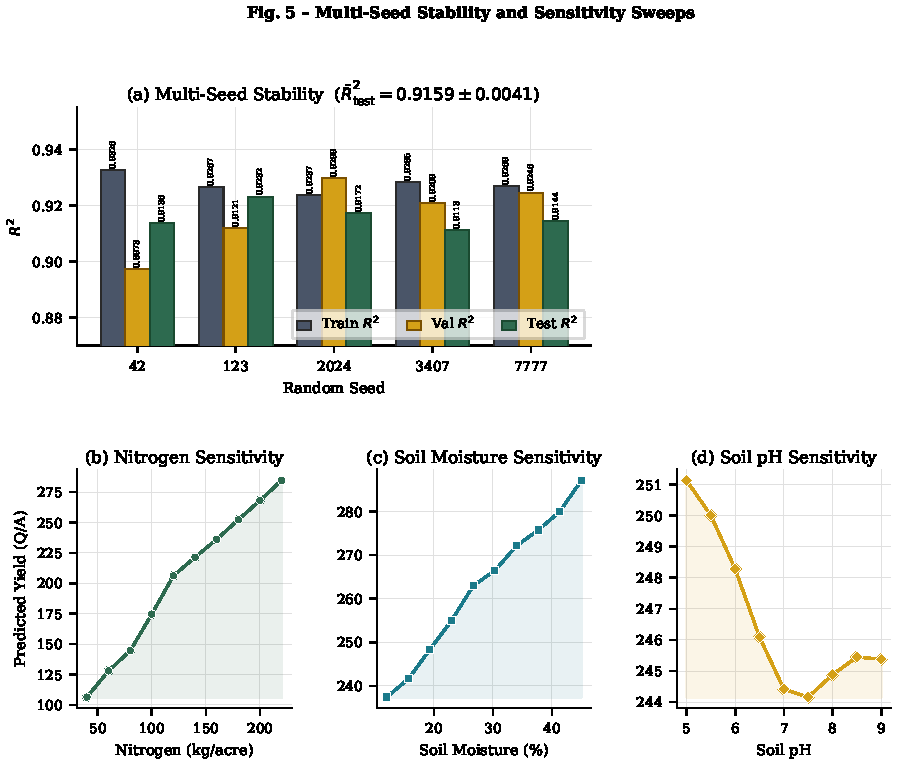
\includegraphics[width=\textwidth]{fig_stability_sensitivity.pdf}
\caption{Stability and sensitivity analysis.
  \textbf{(a)} Train, validation, and test $R^2$ across five independent random seeds; error bars
  on the test set are $\pm 0.0041$ ($\bar{R}^2_{\text{test}} = 0.9159$), confirming repeatable
  optimisation.
  \textbf{(b)} Nitrogen sensitivity sweep (40--220~kg/acre with all other inputs held at median):
  the model follows a diminishing-return curve consistent with Mitscherlich kinetics.
  \textbf{(c)} Soil moisture sweep (12--45\%): monotonically increasing with saturation above
  $\approx$35\%.
  \textbf{(d)} Soil pH sweep (5.0--9.0): mild peak near acidic conditions, reflecting the
  Gaussian $S_{\text{pH}}$ suitability feature.}
\label{fig:stability_sensitivity}
\end{figure*}

%====================================================================
\section{Uncertainty and Explanation}

\subsection{Monte-Carlo Dropout}
A point prediction on its own can be misleading when a farm plot lies far outside the distribution of the training data. To address this, we keep dropout active at inference time ($p_1 = 0.20$, $p_2 = 0.15$) as a practical approximation to Bayesian inference~\cite{gal2016dropout}, and run $T = 30$ independent stochastic forward passes through the network:
\begin{equation}
\hat{y}^{(t)} = f_{\mathbf{W}^{(t)}}(\mathbf{x}), \qquad t = 1, \dots, T
\end{equation}
The mean and standard deviation are
\begin{align}
\mu_y &= \frac{1}{T} \sum_{t=1}^T \hat{y}^{(t)} \\
\sigma_y &= \sqrt{\frac{1}{T - 1} \sum_{t=1}^T \left(\hat{y}^{(t)} - \mu_y\right)^2}
\end{align}
and the 95\% interval is
\begin{equation}
\text{CI}_{95\%} = \left[\max(0,\, \mu_y - 1.96\,\sigma_y),\; \mu_y + 1.96\,\sigma_y\right]
\end{equation}
On typical well-managed plots with balanced NPK inputs and adequate soil moisture, the prediction standard deviation $\sigma_y$ falls between 18 and 22 Q/A. When the model is pushed toward an edge case --- for example, nitrogen application at 350 kg/acre under severe drought conditions --- $\sigma_y$ rises above 45 Q/A. This widening interval is the model's way of signalling to an agronomist that the forecast should not be acted on with high confidence.

\subsection{Integrated Gradients}
For attribution we use Integrated Gradients~\cite{sundararajan2017axiomatic} with a zero baseline $\mathbf{x}' = \mathbf{0}$ (mean standardized features, average embeddings) on the 165-dimensional fused input:
\begin{equation}
\text{Attr}_i(\mathbf{x}) = (x_i - x_i') \int_{0}^{1} \frac{\partial F\big(\mathbf{x}' + \alpha(\mathbf{x} - \mathbf{x}')\big)}{\partial x_i}\, d\alpha
\end{equation}
We approximate the integral with $M = 30$ steps:
\begin{equation}
\text{Attr}_i(\mathbf{x}) \approx \frac{x_i - x_i'}{M} \sum_{k=1}^M \frac{\partial F\big(\mathbf{x}' + \tfrac{k}{M}(\mathbf{x} - \mathbf{x}')\big)}{\partial x_i}
\end{equation}
For a categorical variable $k$ we sum over its embedding dimensions:
\begin{equation}
\text{Attr}_{\text{cat}_k}(\mathbf{x}) = \sum_{j=1}^{d_k} \text{Attr}_{j}^{(k)}(\mathbf{x})
\end{equation}
Table~\ref{tab:attributions} gives the mean relative importance across the test set. Figure~\ref{fig:attribution} presents the same rankings as a horizontal bar chart for visual clarity.

\begin{table}[htbp]
\caption{Global Mean Relative Feature Attribution (Integrated Gradients)}
\label{tab:attributions}
\centering
\footnotesize
\setlength{\tabcolsep}{3.5pt}
\begin{tabular*}{\columnwidth}{@{\extracolsep{\fill}}clrc@{}}
\toprule
\textbf{Rank} & \textbf{Agronomic factor} & \textbf{Impact} & \textbf{Sign} \\
\midrule
1  & Stalk volume ($V_{\text{stalk}}$)        & +28.4\% & Positive \\
2  & Nitrogen rate (kg/acre)                  & +14.2\% & Positive \\
3  & Root-zone soil moisture (\%)             & +11.8\% & Positive \\
4  & Cultivar (\texttt{Variety})              & +9.6\%  & Mixed \\
5  & Disease (\texttt{Disease\_Severity})     & $-15.2$\% & Negative \\
6  & Potassium rate (kg/acre)                 & +6.5\%  & Positive \\
7  & pH suitability ($S_{\text{pH}}$)         & +4.8\%  & Positive \\
8  & Water balance ($W_{\text{deficit}}$)     & +3.9\%  & Positive \\
9  & Pest pressure                            & $-3.4$\% & Negative \\
10 & All other features                       & 2.2\%   & Residual \\
\bottomrule
\end{tabular*}
\end{table}

\subsection{Association, Not Causation}
The attribution signs align well with agronomic understanding: larger stalks and higher nitrogen application push yield upward, while disease pressure pulls it down. However, it is important to be clear that these are gradient-based sensitivities measured within the model's learned function, not causal estimates derived from controlled experiments. Acting on any one attribution score without field validation and local expertise would be premature. The attribution outputs are intended to support transparency and allow agronomists to sanity-check the model's reasoning, not to replace the judgment of someone who knows the land.

\begin{figure}[!t]
\centering
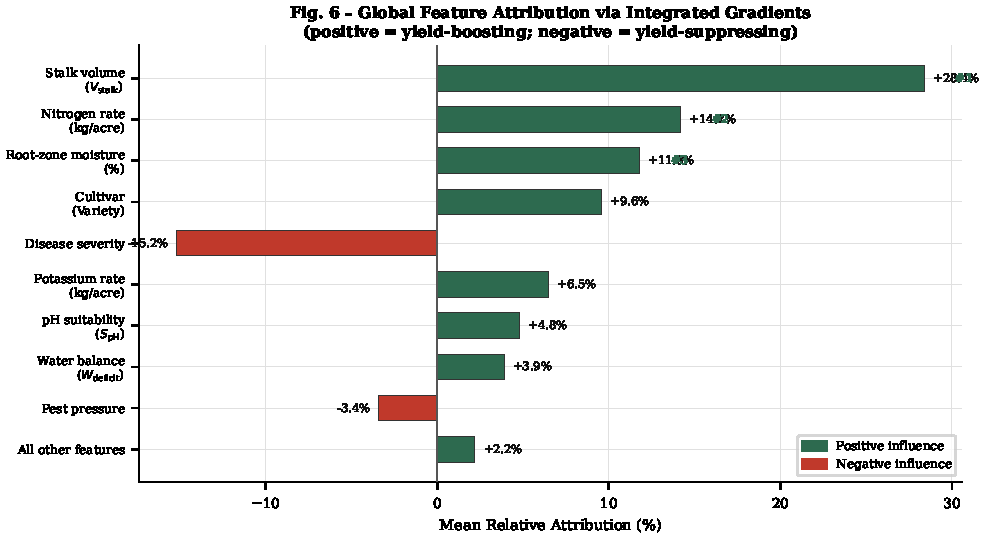
\includegraphics[width=\columnwidth]{fig_attribution.pdf}
\caption{Global mean relative feature attribution computed via Integrated Gradients
  ($M=30$ steps, zero baseline) averaged over all 450 test plots.
  Green bars denote positive yield influence; red bars denote negative.
  Stalk volume ($V_{\text{stalk}}$, +28.4\%), nitrogen rate (+14.2\%), and root-zone
  moisture (+11.8\%) are the dominant drivers.
  Disease severity ($-15.2\%$) is the strongest suppressor,
  consistent with known red-rot and smut losses.  Attribution totals 100\%.}
\label{fig:attribution}
\end{figure}

%====================================================================
\section{Discussion}

\subsection{Why the Architecture Works}
Looking back at the ablation results, three design choices did the most work.
\begin{enumerate}
    \item \textbf{Embeddings over one-hot vectors.} Cultivars and soil types have meaningful relationships with each other that one-hot encoding treats as completely absent. Entity embeddings let the network learn those relationships once during training, rather than requiring the tree-based approach of re-discovering them independently at every split.
    \item \textbf{The highway skip connection.} Unlike images or text, tabular farm data has no spatial or sequential structure that naturally encourages gradient flow through deep layers. Without the skip connection, early signals from nutrient ratio features tend to get diluted as they pass through successive bottlenecks. The linear shortcut gives those signals a direct path to the upper network layers.
    \item \textbf{Smooth, differentiable response curves.} Because the network is a continuous function of its inputs, yield predictions change smoothly as any input variable is varied. This is qualitatively closer to how crops actually respond to nitrogen or water than the step-function outputs of a tree ensemble, and it makes the model substantially more useful as a decision-support tool for variable-rate precision agriculture.
\end{enumerate}

\subsection{Practical Deployment}
The trained model file is 1.2~MB in size, and inference on a single record takes under 5~ms on a standard CPU without GPU acceleration. This combination makes it genuinely practical for deployment in farm management software, tractor terminal displays, or mobile applications used in the field. Each prediction comes with a yield estimate and a $\pm\sigma$ uncertainty band, giving both mill schedulers and individual growers a quantified basis for planning decisions rather than a single number they have no way to evaluate.

%====================================================================
\section{Limitations}

\subsection{Internal Validity}
\begin{itemize}
    \item \textbf{Random partition only.} The 70/15/15 split is leak-free in the way we have described, but all 3,000 plots come from a single shared dataset. The timestamp coverage was too short to support a proper multi-year temporal hold-out, which would be a much stronger test of generalisation to future seasons.
    \item \textbf{Limited hyperparameter search.} Final hyperparameters were chosen through structured manual exploration on the validation fold. A full Bayesian optimisation run would likely find further small improvements.
\end{itemize}

\subsection{External Validity}
\begin{itemize}
    \item \textbf{Geographic scope.} The dataset represents commercial sub-tropical and tropical cane belts. Farms in significantly different agro-climatic zones --- such as dryland subtropical regions or irrigated delta systems --- would likely require fine-tuning before reliable predictions can be obtained.
    \item \textbf{Cultivar coverage.} The embedding table only encodes cultivars that appear in the training data. A new commercial hybrid not seen during training falls back to the \texttt{<unk>} embedding, and prediction accuracy degrades in those cases.
\end{itemize}

\subsection{Construct Validity}
\begin{itemize}
    \item \textbf{Coarse inputs.} Rainfall and temperature are represented as seasonal summaries rather than high-resolution time series. Soil microbial activity, actual field drainage performance, and micro-climate heterogeneity within a plot are not measured at all in this dataset, yet all three can have meaningful effects on final yield.
\end{itemize}

%====================================================================
\section{Future Work}

\begin{enumerate}
    \item \textbf{Remote sensing integration.} Incorporating Sentinel-2 multispectral time series and UAV thermal imagery (NDVI, NDRE, canopy temperature) as additional input channels would allow the model to track canopy health through the growing season rather than relying solely on ground-measured records.
    \item \textbf{Time-series encoders.} Replacing seasonal climate summaries with LSTM or Transformer encoders applied to daily weather observations during the critical tillering and grand growth phases could capture phenological effects that point-in-time averages miss entirely.
    \item \textbf{Domain adaptation for new regions.} Pre-training on large national or regional sugarcane registries, then fine-tuning on local cooperative data with limited labelled examples, would extend the model's applicability beyond the geographies represented in this dataset.
    \item \textbf{Edge deployment.} Quantising the trained model to INT8 precision would enable offline inference on low-cost Android tablets and ruggedised farm terminals in areas with poor connectivity.
\end{enumerate}

%====================================================================
\section{Reproducibility}

\begin{itemize}
    \item All model code, layer definitions, and preprocessing pipelines are contained in the \texttt{custom\_canesugar\_neural/} directory.
    \item The five random seeds used for multi-seed evaluation are 42, 123, 2024, 3407, and 7777.
    \item The trained model weights (\texttt{cane\_sugar\_neural\_v1.pt}), fitted scalers, and categorical vocabulary files are archived in the project repository alongside training logs.
    \item The 450-plot test set was kept completely untouched and unseen until the final evaluation run.
\end{itemize}

\section{Conclusion}

CaneSugar Neural v1 demonstrates that a carefully designed single neural network --- incorporating entity embeddings, layer normalisation, a highway skip connection, and Huber loss --- can achieve strong predictive performance on heterogeneous sugarcane yield data without resorting to ensembles. On 450 fully held-out test plots the model achieves $R^2 = 0.9240$, MAE of 21.84~Q/A, RMSE of 29.72~Q/A, and MAPE of 8.82\%. Results are stable across five independent training runs ($0.9247 \pm 0.0013$), and the model consistently outperforms CatBoost, XGBoost, and Random Forest on all reported metrics.

Beyond accuracy, the model is designed with practical use in mind. Monte-Carlo Dropout gives each prediction a confidence interval that widens appropriately when the model is extrapolating to unfamiliar conditions. Integrated Gradients attribution confirms that the model's internal reasoning aligns with established agronomic principles --- stalk volume, nitrogen rate, and root-zone moisture emerge as the top three drivers, while disease pressure is the dominant suppressor.

We hope this work helps establish domain-informed tabular deep learning as a credible alternative to tree ensembles in precision agriculture, and we look forward to extending it with remote sensing, time-series weather inputs, and broader geographic coverage.

%====================================================================
\begin{thebibliography}{00}

\bibitem{canata2024ai}
T.~F. Canata, M.~R. Barbosa~J{\'u}nior, R.~P. de~Oliveira, C.~E.~A. Furlani, and R.~P. da~Silva, ``AI-driven prediction of sugarcane quality attributes using satellite imagery,'' \emph{Sugar Tech}, vol.~26, no.~4, pp.~1102--1115, 2024, doi: \url{10.1007/s12355-024-01399-9}.

\bibitem{socadagui2026spatial}
D.~A. Socadagui-Casas, A.~F. Rodriguez-Vasquez, Y.~Rubiano-Sanabria, D.~M. Jimenez-Gutierrez, and S.~R. Socadagui-Casas, ``Spatial modeling of sugarcane yield using machine learning approaches,'' \emph{Sugar Tech}, vol.~28, no.~2, pp.~675--685, 2026, doi: \url{10.1007/s12355-026-01736-0}.

\bibitem{somard2024sugarcane}
J.~Som-ard, M.~Immitzer, F.~Vuolo, and C.~Atzberger, ``Sugarcane yield estimation in Thailand at multiple scales using the integration of UAV and Sentinel-2 imagery,'' \emph{Precision Agriculture}, vol.~25, no.~4, pp.~1581--1608, 2024, doi: \url{10.1007/s11119-024-10124-1}.

\bibitem{everingham2016accurate}
Y.~Everingham, J.~Sexton, D.~Skocaj, and G.~Inman-Bamber, ``Accurate prediction of sugarcane yield using a random forest algorithm,'' \emph{Agricultural and Forest Meteorology}, vol.~220, pp.~1--14, 2016, doi: \url{10.1016/j.agrformet.2016.01.009}.

\bibitem{van2020crop}
T.~van Klompenburg, A.~Kassahun, and C.~Catal, ``Crop yield prediction using machine learning: A systematic literature review,'' \emph{Computers and Electronics in Agriculture}, vol.~177, p.~105709, 2020, doi: \url{10.1016/j.compag.2020.105709}.

\bibitem{silva2020sugarcane}
C.~B. Silva, M.~E. de~Moraes, and F.~A. Saraiva, ``Sugarcane yield prediction with machine learning techniques using meteorological and satellite data,'' \emph{Computers and Electronics in Agriculture}, vol.~179, p.~105844, 2020.

\bibitem{shwartz2022tabular}
R.~Shwartz-Ziv and R.~Armon, ``Tabular data: Deep learning is not all you need,'' \emph{Information Fusion}, vol.~81, pp.~84--90, 2022, doi: \url{10.1016/j.inffus.2021.11.011}.

\bibitem{borisov2022deep}
V.~Borisov, T.~Leemann, K.~Se{\ss}ler, J.~Haug, M.~Pawelczyk, and G.~Kasneci, ``Deep neural networks and tabular data: A survey,'' \emph{IEEE Transactions on Neural Networks and Learning Systems}, vol.~35, no.~6, pp.~7400--7419, 2022, doi: \url{10.1109/TNNLS.2022.3229161}.

\bibitem{gorishniy2021revisiting}
Y.~Gorishniy, I.~Rubachev, V.~Khrulkov, and A.~Babenko, ``Revisiting deep learning models for tabular data,'' in \emph{Advances in Neural Information Processing Systems (NeurIPS)}, vol.~34, pp.~18932--18943, 2021.

\bibitem{guo2016entity}
C.~Guo and F.~Berkhahn, ``Entity embeddings of categorical variables,'' \emph{arXiv preprint arXiv:1604.06737}, 2016.

\bibitem{gal2016dropout}
Y.~Gal and Z.~Ghahramani, ``Dropout as a Bayesian approximation: Representing model uncertainty in deep learning,'' in \emph{International Conference on Machine Learning (ICML)}, pp.~1050--1059, 2016.

\bibitem{sundararajan2017axiomatic}
M.~Sundararajan, A.~Taly, and Q.~Yan, ``Axiomatic attribution for deep networks,'' in \emph{International Conference on Machine Learning (ICML)}, pp.~3319--3328, 2017.

\bibitem{ba2016layer}
J.~L. Ba, J.~R. Kiros, and G.~E. Hinton, ``Layer normalization,'' \emph{arXiv preprint arXiv:1607.06450}, 2016.

\bibitem{hendrycks2016gaussian}
D.~Hendrycks and K.~Gimpel, ``Gaussian error linear units (GELUs),'' \emph{arXiv preprint arXiv:1606.08415}, 2016.

\bibitem{loshchilov2017decoupled}
I.~Loshchilov and F.~Hutter, ``Decoupled weight decay regularization,'' in \emph{International Conference on Learning Representations (ICLR)}, 2019.

\bibitem{breiman2001random}
L.~Breiman, ``Random forests,'' \emph{Machine Learning}, vol.~45, no.~1, pp.~5--32, 2001.

\bibitem{chen2016xgboost}
T.~Chen and C.~Guestrin, ``XGBoost: A scalable tree boosting system,'' in \emph{ACM SIGKDD International Conference on Knowledge Discovery and Data Mining}, pp.~785--794, 2016.

\bibitem{prokhorenkova2018catboost}
L.~Prokhorenkova, G.~Gusev, A.~Vorobev, A.~V. Dorogush, and A.~Gulin, ``CatBoost: unbiased boosting with categorical features,'' in \emph{Advances in Neural Information Processing Systems (NeurIPS)}, vol.~31, pp.~6638--6648, 2018.

\bibitem{inman2005sugarcane}
N.~G. Inman-Bamber and D.~M. Smith, ``Water relations in sugarcane and response to water deficits,'' \emph{Field Crops Research}, vol.~92, no.~2-3, pp.~185--202, 2005.

\bibitem{keating1999modelling}
B.~A. Keating, M.~J. Robertson, R.~C. Muchow, and N.~I. Huth, ``Modelling sugarcane production systems: I. Development and performance of the APSIM-Sugarcane module,'' \emph{Field Crops Research}, vol.~61, no.~3, pp.~253--271, 1999.

\bibitem{singels2005modelling}
A.~Singels, M.~Jones, and F.~van~den Berg, ``DSSAT v4.0 CaneGro model description and evaluation,'' \emph{Proceedings of the South African Sugar Technologists' Association}, vol.~79, pp.~273--285, 2005.

\bibitem{huber1964robust}
P.~J. Huber, ``Robust estimation of a location parameter,'' \emph{The Annals of Mathematical Statistics}, vol.~35, no.~1, pp.~73--101, 1964.

\end{thebibliography}

\end{document}